\documentclass[10pt,twocolumn]{article}

\usepackage[margin=0.72in,columnsep=0.24in]{geometry}
\usepackage[T1]{fontenc}
\usepackage{lmodern}
\usepackage{microtype}
\usepackage{amsmath,amssymb}
\usepackage{booktabs}
\usepackage{graphicx}
\usepackage[numbers,sort&compress]{natbib}
\usepackage[colorlinks=true,allcolors=blue]{hyperref}

\setlength{\emergencystretch}{2em}
\graphicspath{{figures/}}
\hypersetup{
  pdftitle={Token Identity as a Routing Signal for Residual MLP Experts},
  pdfauthor={Boris Peyriguere},
  pdfsubject={Deterministic token-ID routing for residual MLP experts},
  pdfkeywords={language models, mixture of experts, deterministic routing}
}

\title{\textbf{Token Identity as a Routing Signal\\for Residual MLP Experts}}
\author{
  Boris Peyriguere\\
  Complexity-ML, Independent Research\\
  \texttt{boris@complexity-ai.fr}
}
\date{July 2026}

\newcommand{\trmodel}{token-routed}
\newcommand{\MhaTRSeedB}{7.541488}
\newcommand{\MhaTRPPLSeedB}{1884.63}
\newcommand{\MhaDeltaSeedB}{-0.185483}

\begin{document}
\maketitle

\begin{abstract}
Mixture-of-experts language models normally learn routing decisions from
contextual hidden states. We study a narrower question: can token identity
select a useful residual parameter subspace when a shared dense MLP remains
active for every token? A fixed layer-specific lookup selects two narrow
experts, while the shared branch and selected experts transform the same
contextual hidden state. In a parameter- and token-matched single-seed
comparison, 306.5M-parameter models are trained on 8B FineWeb-Edu tokens. The
\trmodel{} model reaches diagnostic-stream negative log-likelihood (NLL)
2.9329 versus 2.9482 for dense, but trains 21\% more slowly. Independent-corpus
evaluation changes ordering: routing is ahead on C4 validation and dense is
ahead on a Pile test subset. Small Apple-MPS pilots additionally compare dense
and routed feed-forward paths under both grouped-query and full multi-head
attention. Their paired differences favor routing across the completed runs,
but the pilots recycle a small local corpus and are not evidence of scaling or
generalization. The results support token identity as a useful experimental
routing signal, not as a general replacement for contextual routing.
\end{abstract}

\section{Introduction}

Sparse language models typically learn a router that maps each contextual
hidden state to a subset of experts
\citep{shazeer2017outrageously,fedus2022switch,jiang2024mixtral}. This combines
two questions: whether conditional capacity is useful and whether a learned
contextual decision is required to select it. Fixed routing separates these
questions. Hash Layers showed that simple hashes of local token features can
be competitive routing signals \citep{roller2021hash}; shared-expert systems
suggest that common computation can remain dense while specialization is
sparse \citep{dai2024deepseekmoe}.

We test a deliberately asymmetric design. Every token traverses a shared
SwiGLU MLP. Token identity selects two additional narrow residual experts.
Selection is context independent, but expert computation is not: both paths
receive the contextual hidden state produced by attention. The study asks
whether lexical identity can allocate a residual parameter subspace, not
whether token IDs can replace contextual sequence processing.

Our main evidence is a matched 306.5M-parameter, 8B-token run pair. We report
the complete scope of that observation, including slower routed training and
opposite ordering on two independent corpora. We then add bounded local pilots
that test whether the shared-plus-routed feed-forward design behaves similarly
with grouped-query attention (GQA) and multi-head attention (MHA).

\section{Architecture}

\begin{figure*}[t]
\centering
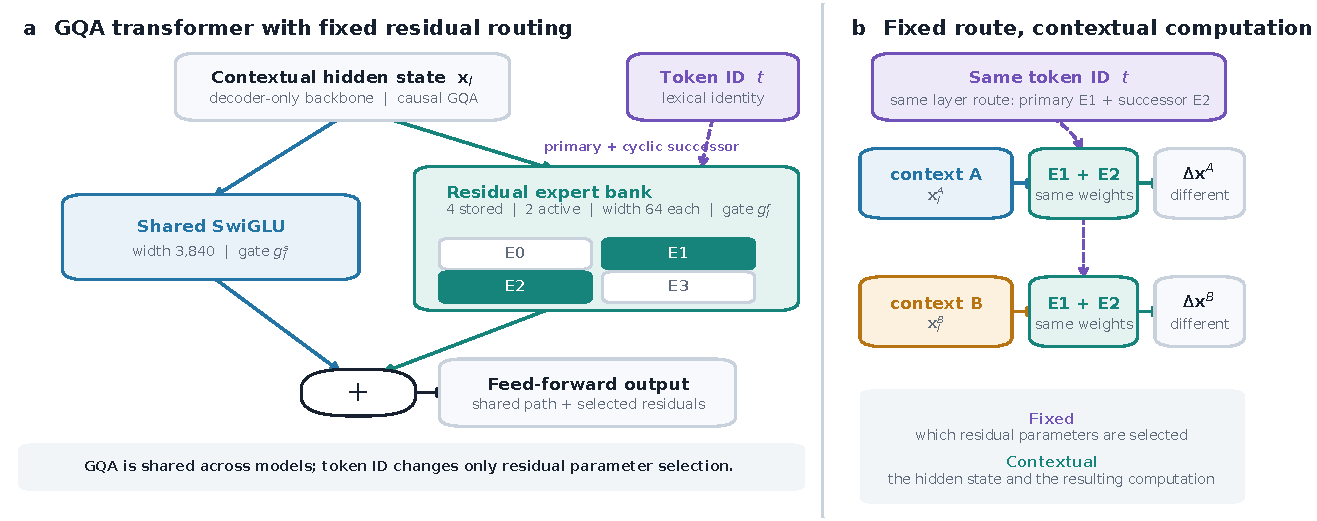
\includegraphics[width=0.86\textwidth]{architecture_complexity_deep.pdf}
\caption{\textbf{Token identity controls parameter selection, not contextual
computation.} Attention produces contextual hidden state $\mathbf{x}$. Every
token traverses the shared SwiGLU branch. A fixed layer-specific table maps
token identifier $t$ to two narrow residual experts, which also transform
$\mathbf{x}$.}
\label{fig:architecture}
\end{figure*}

For layer $l$, token ID $t$, and $E=4$ stored experts, the primary experiment
uses a seeded permutation of the token-ID residue,
\begin{equation}
r_{l,1}(t)=\pi_l(t\bmod E),
\end{equation}
with cyclic secondary route
\begin{equation}
r_{l,2}(t)=\bigl(r_{l,1}(t)+1\bigr)\bmod E.
\end{equation}
The feed-forward output is
\begin{equation}
\begin{split}
\operatorname{FFN}_l(\mathbf{x},t)
={}&g_l^s\,\operatorname{Shared}_l(\mathbf{x})\\
&+g_l^r\sum_{j=1}^{2}0.5\,
\operatorname{Expert}_{r_{l,j}(t)}(\mathbf{x}),
\end{split}
\end{equation}
where shared and expert branches are SwiGLU transformations. The primary model
learns scalar branch gates initialized to $0.5$. The lookup has no learned
router and receives no contextual state.

Let $d_s$ be shared width, $d_e$ expert width, $E$ the number of stored
experts, and $k$ the number selected. Ignoring biases, stored intermediate
width is $d_s+Ed_e$, while active width is $d_s+kd_e$. The primary routed model
uses $(d_s,E,d_e,k)=(3840,4,64,2)$, so its stored width matches the dense width
of 4096 while its active width is 3968.

\section{Primary 306.5M experiment}

\subsection{Protocol}

The dense and routed models share an 18-layer decoder-only transformer,
dimension 1024, 16 query heads, four key/value heads, QK-Norm, RoPE, a
32,000-token vocabulary, and context length 2048. They use the same
FineWeb-Edu order, AdamW configuration, schedule, BF16 precision, and 8B-token
budget. Each model contains 306.5M parameters. The comparison has one seed per
architecture.

\subsection{Matched-token result}

\begin{table}[t]
\centering
\small
\caption{Primary matched comparison. Lower NLL is better.}
\label{tab:primary}
\begin{tabular}{lrr}
\toprule
Measurement & Dense & Token-routed \\
\midrule
Eval-stream NLL & 2.9482 & \textbf{2.9329} \\
Final train NLL & 2.9324 & \textbf{2.9231} \\
Training throughput & \textbf{$\sim$0.95M} & $\sim$0.75M \\
\bottomrule
\end{tabular}
\end{table}

At the last common diagnostic checkpoint, after 7.864B processed tokens, the
routed model is ahead by $0.0153$ NLL (Table~\ref{tab:primary}). The diagnostic
stream is fixed across models but drawn from the FineWeb-Edu training split;
it is not held out. Routed training is approximately 21\% slower in the
reported implementation.

\subsection{Independent-corpus evaluation}

\begin{table}[t]
\centering
\small
\caption{Independent-corpus NLL of the final checkpoints. Each row scores
262,144 targets in paired blocks.}
\label{tab:heldout}
\begin{tabular}{lrrr}
\toprule
Corpus & Dense & Routed & $\Delta$ \\
\midrule
C4 validation & 3.4161 & \textbf{3.4066} & $-0.0095$ \\
Pile test subset & \textbf{2.8690} & 2.8769 & $+0.0079$ \\
\bottomrule
\end{tabular}
\end{table}

C4 favors routing, while the Pile subset favors dense
(Table~\ref{tab:heldout}). No decontamination against FineWeb-Edu was
performed. These measurements demonstrate corpus-dependent ordering rather
than a universal generalization advantage.

\section{Local Apple-MPS pilots}

\subsection{Purpose and protocol}

The local pilots test the feed-forward design under two attention backbones.
They are intentionally small architecture checks, not replications of the
8B-token experiment. Every run has 99,487,680 parameters, hidden size 384, 10
layers, eight query heads, and a 200,019-token o200k vocabulary. GQA uses two
key/value heads; MHA uses eight. Each run trains for 250 steps with batch size
4 and sequence length 1024, totaling 1,024,000 sampled training tokens.

The source is a local 400-document FineWeb-Edu sample containing 356,120
tokens. A deterministic 95/5 split leaves 338,314 training tokens and 17,806
evaluation-tail tokens. Training therefore resamples the small training
partition. Route frequencies are computed from the training partition only.
Evaluation uses four batches sampled from the fixed tail, paired within each
seed. All runs use AdamW with learning rate $3\times10^{-4}$, weight decay
0.1, and Apple MPS with PyTorch fallback kernels.

The local routed variant uses modulo-primary routing with a
training-frequency-balanced secondary assignment, fixed top-2 weights
$0.5/0.5$, and no learned shared/routed gate. GQA allocates stored FFN width
$1392+256$ between shared and routed paths; its dense control uses width 1648.
MHA allocates $1296+160$; its dense control uses width 1456. The differences
preserve the same total parameter count within each paired comparison.

\begin{table*}[t]
\centering
\small
\caption{\textbf{Matched local Apple-MPS pilots.} $\Delta$ is routed minus
dense evaluation NLL within the same attention type and seed. Lower is better.
The two seeds use the same split but different initialization and evaluation
sampling seeds.}
\label{tab:mps}
\begin{tabular}{llrrrrr}
\toprule
Attention & Seed & Dense NLL & Routed NLL & Dense PPL & Routed PPL & $\Delta$ NLL \\
\midrule
GQA & 42 & 7.596686 & \textbf{7.536167} & 1991.58 & \textbf{1874.63} & $-0.060519$ \\
GQA & 43 & 7.530082 & \textbf{7.492290} & 1863.26 & \textbf{1794.16} & $-0.037792$ \\
MHA & 42 & 7.586145 & \textbf{7.536471} & 1970.70 & \textbf{1875.20} & $-0.049674$ \\
MHA & 43 & 7.726971 & \textbf{\MhaTRSeedB} & 2268.72 & \textbf{\MhaTRPPLSeedB} & $\MhaDeltaSeedB$ \\
\bottomrule
\end{tabular}
\end{table*}

All four paired runs favor the routed feed-forward path
(Table~\ref{tab:mps}). The mean paired NLL difference is $-0.049156$ for GQA
and $-0.117579$ for MHA. The substantial variation between MHA seeds cautions
against interpreting either mean as a precise effect estimate. Current median
logged MPS throughput is lower for routed
models: 4708 versus 5418.5 tokens/s for GQA, and 4398.5 versus 5590.5 tokens/s
for MHA at seed 42. These fallback measurements are implementation-specific
and are not CUDA deployment benchmarks.

\section{Limitations}

The primary result has one seed per architecture. Its training-time diagnostic
stream is not held out, and independent corpora change model ordering. The
local pilots use two initialization seeds at most, recycle a small training
partition, score only four sampled evaluation batches, and use an updated
secondary assignment rather than the exact cyclic mapping of the primary
model. Their widths were selected during local exploration. They therefore
test implementation behavior and direction, not statistical significance,
large-scale persistence, or downstream capability.

The strongest next tests are predeclared multi-seed training on a larger
shard, frozen-checkpoint evaluation on separate corpora, equal-compute
comparisons, and optimized sparse kernels. Learned contextual routers remain
an important control: this work does not claim that fixed routing is generally
superior to learned routing.

\section{Conclusion}

Token identity can provide a useful fixed signal for selecting narrow residual
MLP experts while a shared dense path preserves common contextual computation.
The 306.5M run pair shows a modest matched-token advantage but slower training
and corpus-dependent generalization. Small local pilots show the same
short-budget direction under both GQA and MHA, subject to much stronger
limitations. The evidence motivates controlled replication rather than a
claim of a universally better routing architecture.

\paragraph{Reproducibility.}
Code, configurations, model cards, and machine-readable metrics are available
at \url{https://github.com/Complexity-ML/complexity-framework}. The primary
checkpoints are available at
\url{https://huggingface.co/Pacific-i64/TR-MOE-306} and
\url{https://huggingface.co/Pacific-i64/Dense-306}.

\paragraph{Use of generative AI tools.}
Generative AI tools assisted with language editing, consistency checks against
author-provided metric files, figure scripting, and packaging. The author
reviewed the numerical results, claims, source, and final text and takes
responsibility for the work.

\bibliographystyle{plainnat}
\bibliography{references}

\end{document}
